\documentclass[11pt]{exam}

\oddsidemargin=0.25truein \evensidemargin=0.25truein
\topmargin=-0.5truein \textwidth=6.0truein \textheight=8.75truein

%\RequirePackage{graphicx}
\usepackage{comment}
\usepackage{verbatim}
\usepackage{booktabs}
\usepackage{graphicx}
\usepackage{hyperref}
\urlstyle{rm}   % change fonts for url's (from Chad Jones)
\hypersetup{
    colorlinks=true,        % kills boxes
    allcolors=blue,
    pdfsubject={ECON-UB233, Macroeconomic foundations for asset pricing},
    pdfauthor={Dave Backus @ NYU},
    pdfstartview={FitH},
    pdfpagemode={UseNone},
%    pdfnewwindow=true,      % links in new window
%    linkcolor=blue,         % color of internal links
%    citecolor=blue,         % color of links to bibliography
%    filecolor=blue,         % color of file links
%    urlcolor=blue           % color of external links
% see:  http://www.tug.org/applications/hyperref/manual.html
}

\renewcommand{\thefootnote}{\fnsymbol{footnote}}
\newcommand{\var}{\mbox{\it Var\/}}

\usepackage{attachfile}
    \attachfilesetup{color=0.5 0 0.5}

\usepackage{enumitem}
\setitemize{leftmargin=*, topsep=0pt}
\setenumerate{leftmargin=*, topsep=0pt}

\printanswers

% document starts here
\begin{document}
\parskip=\bigskipamount
\parindent=0.0in
\thispagestyle{empty}
{\large ECON-UB 233 \hfill Dave Backus @ NYU}

\bigskip\bigskip
\centerline{\Large \bf Lab Report \#6: Options \& Volatility}
\centerline{Revised: \today}

\bigskip
{\it Due at the start of class.
You may speak to others, but whatever you hand in should be your own work.
Please include your Matlab code.

I suspect some people will find the programming parts of this
somewhat demanding.  If so, do questions 1 and 2 and stop.
And come see me if you have questions.
}

\begin{solution}
Brief answers follow,
but see also the attached Matlab program;
download the pdf, open, click on pushpin:
\attachfile{../Matlab/hw/hw6_f13.m}
\end{solution}

\begin{questions}
%-----------------------------------------------------------------------
\question {\it Root-finding.\/}
Consider the function $f(x) = x \cos(x) $.
Our mission is to find solutions $x^*$
between one and two for which $f(x) = 0$.
%
\begin{parts}
\item Plot $f$ against  a grid of points $x$ between one and two.
How many solutions do you see?
\item Write or adapt a Newton's method program to find a solution.
What is it?
\item Change the function to $f(x) = x \cos(x) - c$.
Modify your program to find solutions
for $ c = (1/2, 0, -1/2)$.
What are they?
Can you get your program to find them all at once?
\end{parts}
{\it Comment: I find it useful to define $f$
as a so-called ``anonymous function'' in Matlab: \\
{\tt f = @(x) x.*cos(x) - c }\\
The first part ({\tt f = @(x)}) defines $f$ as a function of $x$.
The rest gives us the function.
The {\tt .*} operator allows this to work for vectors, too.
Doing it this way allows us to define the function once,
then write {\tt f(x)} whenever we want to use it.
For examples, see the
\href{http://pages.stern.nyu.edu/~dbackus/233/root_finding_pjb.m}{Matlab code}
posted on the course outline.
}

\begin{solution}
\begin{parts}
\item The function is monotonic in this interval
and crosses the axis once.
\item The solution is 1.5708.
\item For the vector of values for $c$,
the solutions are $( 1.0980, 1.5708, 1.8452)$.
\end{parts}
\end{solution}

%-----------------------------------------------------------------------
\question {\it Black-Scholes-Merton formula.\/}
We'll examine the BSM formula in some numerical examples.
In what follows, the current price of the underlying
is 102, the option maturity is one year, and the one-year bond price is 0.95.
\begin{parts}
\part If volatility $\sigma = 0.10$,
what are the prices of call options at strike prices
of 90, 100, and 110?
Why do they decline with the strike price?
\part What are the prices of put options with the same strikes?
\part If volatility rises to $\sigma = 0.125$,
what happens to the prices of calls?
\part For strikes of 90, 100, and 110,
graph the call price against volatility $\sigma$
using a grid between (roughly) 0.01 and 0.50.
(This gives you three lines, one for each strike.)
How do call prices vary with volatility?
Does the pattern vary with the strike price?
\part For a strike of 110 and a call price of 3.50,
what is the implied value of $\sigma$?
\end{parts}

\begin{solution}
\begin{parts}
\part Call prices are 16.65, 8.38, and 2.99 at strikes
of 90, 100, and 110, resp.
They decline because the cash flows are lower at all outcomes $s_{t+1}$.
[Draw a graph of $ (s_{t+1} - k)^+ $ v. $s_{t+1}$ for two values of $k$.]

\part For put options, the easiest route is to use put-call parity.
The put prices are 0.15, 1.38, and 5.49.

\part Calls rise to 16.92, 9.18, and 3.99.
Why rise?  Options prices are increasing in $\sigma$.
We can show this by differentiating the function or by plotting
it, as we do next.

\part See the Matlab program.
You see that call prices increase with volatility in all cases.
(Puts, too, for that matter.)
The relation is close to linear except for very small values of $\sigma$.
(Think about the value of an option as $\sigma$ approaches zero.)

\part From the values computed for the figure, $\sigma = 0.113$ is about it.
\end{parts}
\end{solution}


%-----------------------------------------------------------------------
\question {\it Volatilities for S\&P 500 E-mini options.\/}
For E-mini options,
the prices are more conveniently expressed in
terms of their implied volatilities.
We'll compute them here for quotes reported on March 15, 2012:

\begin{center}
\tabcolsep=0.15in
\begin{tabular}{lcccc}
\toprule
      &  \multicolumn{2}{c}{Call Price} &  \multicolumn{2}{c}{Put Price}  \\
Strike    &  Bid & Ask &  Bid & Ask  \\
\midrule
1340  & 82.50 & 85.75 & 28.25 & 30.25 \\
1350  & 75.25 & 78.25 & 30.75 & 32.75 \\
1360  & 68.00 & 71.00 & 33.25 & 35.50  \\
1370  & 61.25 & 64.00 & 36.25 & 38.75 \\
1380  & 54.50 & 57.25 & 39.50 & 42.25 \\
1390  & 48.25 & 50.75 & 43.25 & 45.75  \\
1400  & 42.25 & 44.75 & 47.00 & 50.00  \\
1410  & 36.75 & 39.25 & 51.25 & 54.50   \\
1420  & 31.75 & 33.75 & 56.00 & 59.25 \\
1430  & 27.00 & 29.00 & 61.25 & 64.50  \\
\bottomrule
\end{tabular}
\end{center}
The price of the underlying contract was 1395.75.
The interest rate was essentially zero, so the appropriate bond price was one.
The options expire June 15, so $\tau = 3/12 = 1/4 $.

\begin{parts}
\item Compute ``mid'' quotes as averages of bid and ask.
Use put-call parity to compute call prices from mid puts.
Plot call prices --- bid, ask, and implied by puts ---
against the strike.
How do they compare?

\item Write a Newton's method program
to compute implied volatilities for mid quotes of call options.
Graph them against the strike.
What shape does the resulting ``smile'' have?
What does the shape suggest to you about the risk-neutral probabilities?
\end{parts}
{\it Comments:
\begin{itemize}
\item If you're lazy like me, you can look up the derivative in Wikipedia.
They refer to the derivative of the call price with respect to volatility
as ``vega.''
You can calculate the derivative with an anonymous function, too,
just as we did in the Newton's method example posted on the course outline.
\item I use this two-step definition of the BSM formula:
\begin{verbatim}
d = @(sigma,k) (log(s./(q_tau.*k))+tau*sigma.^2/2)./(sqrt(tau)*sigma);
f = @(sigma,k) q*normcdf(d(sigma,k)) - ...
        q_tau.*k.*normcdf(d(sigma,k)-sqrt(tau)*sigma) - call_mid;
fp = @(d) s*sqrt(tau)*exp(-d.^2/2)/sqrt(2*pi);
\end{verbatim}
Here we've subtracted the call price from the formula to give us a
function {\tt f} whose value is zero when we find the right volatility.
\item We can do the same with the vega:
\begin{verbatim}
fp = @(d) s*sqrt(tau)*exp(-d.^2/2)/sqrt(2*pi);
\end{verbatim}
\end{itemize}
}

\begin{solution}
\begin{parts}
\item
Run the Matlab program for the figure.
Call prices computed from mid puts (asterisks)
are within the bid-ask spread for call prices,
so evidently people in this market understand
the arbitrage possibilities from violations of put-call parity.

\item This is a more involved calculation.
The idea is to use a vectorized version of Newton's method to
compute implied volatilities from call prices.
One useful input is the derivative of the call price with respect
to volatility:
\begin{eqnarray*}
    \partial q^c/\partial \sigma &=& s \ p(d) \ \tau^{1/2} ,
\end{eqnarray*}
where $p(d) = (2 \pi)^{-1/2} \exp(-d^2/2) $ is the normal pdf
and $d$ is the usual component of the BSM formula.
You can look this up in 
\href{http://en.wikipedia.org/wiki/Black-Scholes#The_Greeks}{Wikipedia}.  

In the figure plotted by the Matlab program,
we see that implied vols decline with strike.
That means prices at low strikes are relatively more expensive than the BSM formula
with constant $\sigma$ would suggest.
If you did this for a broader range of maturities,
you would also see some convexity in the smile.

%\begin{center}
%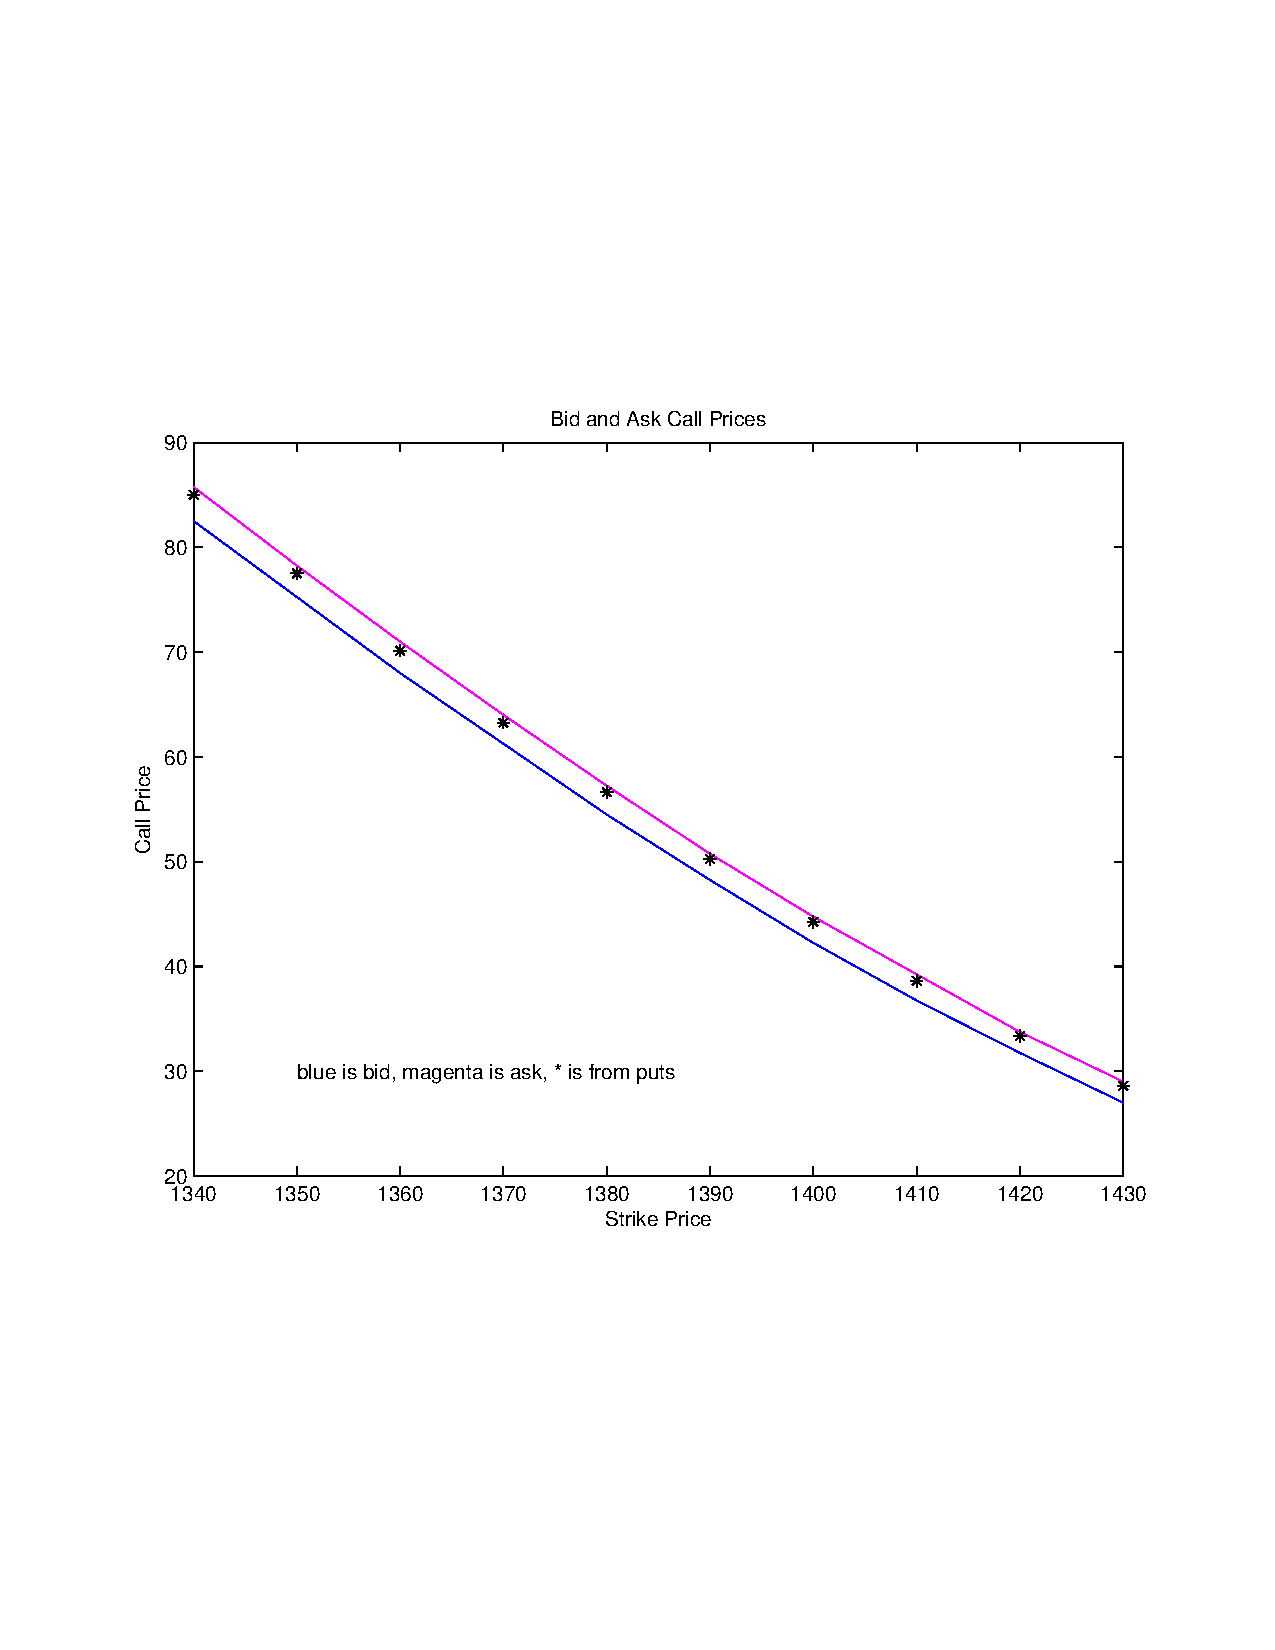
\includegraphics[width=4in]{../Matlab/hw6_q2a.pdf} \\
%%\end{center}
%%\begin{center}
%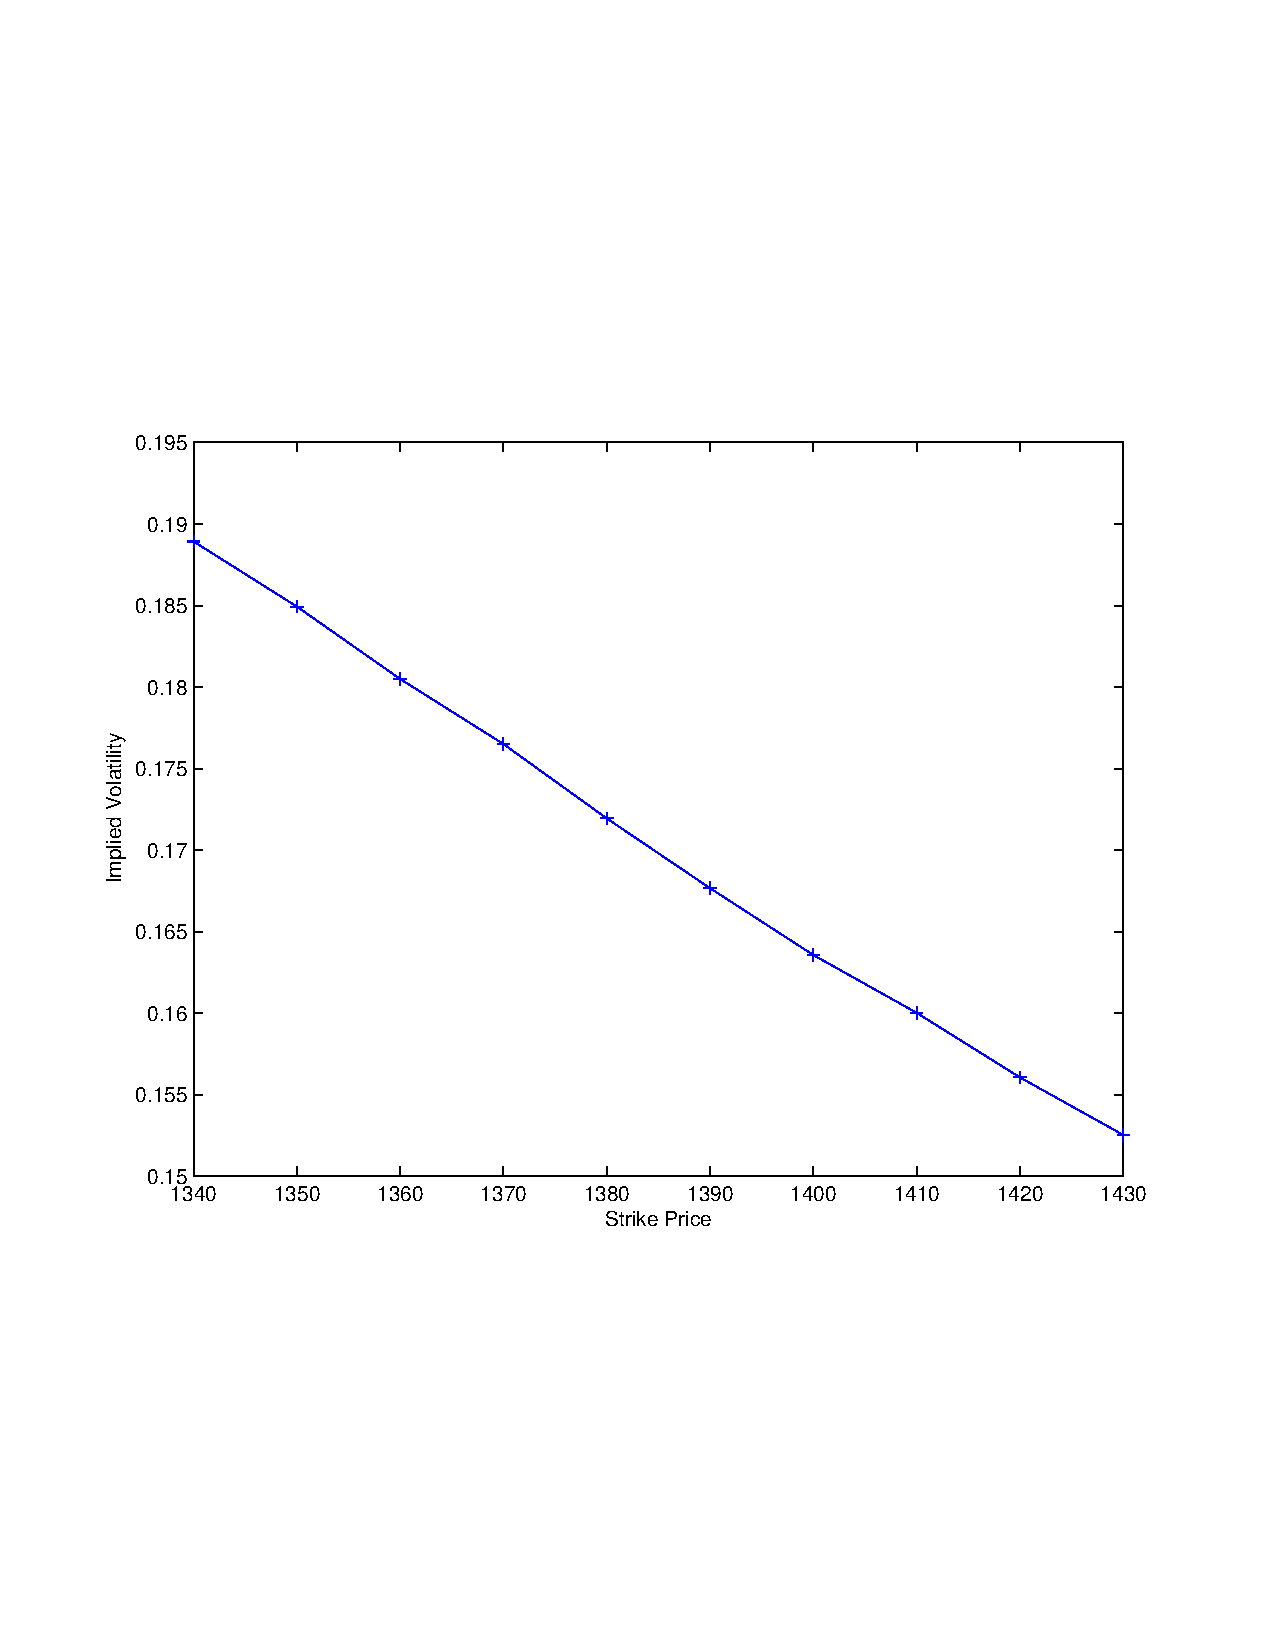
\includegraphics[width=4in]{../Matlab/hw6_q2b.pdf}
%\end{center}

% option prices
%\url{http://www.cmegroup.com/trading/equity-index/us-index/e-mini-sandp500.html}.
\end{parts}
\end{solution}

\end{questions}

\vfill \centerline{\it \copyright \ \number\year \ NYU Stern School of Business}

\end{document}


%-----------------------------------------------------------------------
\question {\it Sums and mixtures (review).\/}
Let us say that the log-price of the underlying has two components:
\begin{eqnarray*}
    \log s_{t+1} &=& y_{t+1} \;\;=\;\; x_{1t+1} + x_{2t+1},
\end{eqnarray*}
with $( x_{1t+1}, x_{2t+1})$ independent.
The first component is normal:
$ x_{1t+1} \sim \mathcal{N}(\mu,\sigma^2)$.
The second component, the ``jump,'' is a mixture:
with probability $1-\omega$, $ x_{2t+1} = 0$,
and with probability $\omega$,
$ x_{2t+1} \sim \mathcal{N}(\theta,\delta^2)$.

With these inputs, the pdf for $y$ is a weighted average of normals:
\begin{eqnarray}
    p(y) &=& (1-\omega) \cdot ( 2 \pi \sigma^2)^{-1/2} \exp[ - (y-\mu)^2/2\sigma^2]
            \nonumber \\
    && + \; \omega \cdot [ 2 \pi (\sigma^2+\delta^2)]^{-1/2}
            \exp[ - [y-(\mu+\theta)]^2/2(\sigma^2 + \delta^2)] .
            \label{eq:bernoulli-mixture}
\end{eqnarray}
If $\omega = 0$, the second component drops out.
Otherwise, we have a weighted average of two normal densities.

\begin{parts}
\part Show that the cumulant generating function for $x_{1t+1}$ is
\begin{eqnarray*}
    k (s; x_1) &=&  \mu s + \sigma^2 s^2 / 2 .
\end{eqnarray*}

\part Show that the cumulant generating function for $x_{2t+1}$ is
\begin{eqnarray*}
    k (s; x_2) &=& \log \left[ (1-\omega) + \omega e^{ \theta s + \delta^2 s^2 / 2 }
            \right] .
\end{eqnarray*}

\part What is the cgf for $y_{t+1}$?
What are its mean, variance, skewness, and excess kurtosis?
What parameters determine the sign of skewness?
\end{parts}

\begin{solution}
The overall idea here is that this construction
can give us useful departures from a normal distribution.
Details follow from applying the usual methods.
\begin{parts}
\part  The usual normal cgf.
\part This is a Bernoulli mixture with one twist:
the ``$\omega$ branch'' has a normal mgf in it.
If $\delta = 0$, it's just like the Bernoulli we looked at in
Lab Report \#1.
Otherwise, we get some additional terms.

\part The cgf of the sum is the sum of the cgfs:
\begin{eqnarray*}
        k (s; y) &=& k (s; x_1) + k (s; x_2) \\
             &=& ( \mu s + \sigma^2 s^2 / 2 ) +
              \log \left[ (1-\omega) + \omega e^{ \theta s + \delta^2 s^2 / 2 }
            \right] .
\end{eqnarray*}
We find it cumulants from derivatives, which are conveniently
computed by Matlab.
The mean and variance are
\begin{eqnarray*}
    \kappa_1 &=& \mu + \omega \theta \\
    \kappa_2 &=& \sigma^2 + \omega (1-\omega) \theta^2 + \omega \delta^2 .
\end{eqnarray*}
Each has terms from each component.
The third and fourth cumulants come only from $x_2$, because the normal
component has zero cumulants beyond the first two.
The third one is
\begin{eqnarray*}
    \kappa_3 &=& \omega (1-\omega) \theta [ 3 \delta^2 + (1-2\omega) \theta^2]  \\
    \kappa_4 &=& \omega (1-\omega)
        \{  \theta^4 [1 - 6 \omega(1-\omega)] + 3 \delta^4 + (1-2 \omega) 6 \delta^2 \theta^2
        \}
\end{eqnarray*}
This is a bit of a mess, but for $\omega$ small,
$\kappa_3$ depends on the sign of $\theta$
and $\kappa_4 >0 $,
so the mixture introduces skewness and excess kurtosis,
both of which are absent from normal random variables.

\part We know normal pfd's integrate to one.
The is a weighted average of normal pdf's, so it must
integrate to one as well.
\end{parts}
\end{solution}


%-----------------------------------------------------------------------
\question {\it Merton-like option pricing.\/}
With the same setup, we can illustrate the value of mixtures in
generating nonnormal distributions and
their impact on option prices and volatility smiles.

\begin{parts}
\part Risk-neutral asset pricing tells us, in general, that
\begin{eqnarray*}
    s_t &=& q^1_t E^* (s_{t+1} )
            \;\;=\;\; q^1_t E^* \left( e^{y_{t+1}}\right)
            \;\;=\;\; q^1_t  e^{k(1; y)}  .
\end{eqnarray*}
We refer to this as the no-arbitrage condition.
What is the no-arbitrage condition for our example?

We'll use this condition to set $\mu$:
given values for everything else, we'll choose $\mu$ to satisfy this condition.

\part Recall that if the risk-neutral distribution is
 $\log s_{t+1} = y_{t+1} \sim \mathcal{N}(\kappa_1,\kappa_2)$,
 then the put price at strike $k$ is
\begin{eqnarray*}
    f(k; \kappa_1, \kappa_2) &=& q^1_t k N(d) - q^1_t e^{\kappa_1 + \kappa_2/2}
            N(d-\kappa_2^{1/2}) \\
            d&=& (\log k - \kappa_1)/\kappa_2^{1/2} .
\end{eqnarray*}
(Note:  this isn't quite the usual $d$.)
What is the call price?

\part
Use (b) to show that the put price in the mixture model is a weighted average:
\begin{eqnarray*}
    q^p_t &=& (1-\omega) \cdot f(k; \mu, \sigma^2) +
        \omega \cdot f(k; \mu+\theta, \sigma^2 + \delta^2) .
\end{eqnarray*}

\part Consider these inputs:
$\sigma = 0.04$, $\omega = 0.01$,
$\theta = -0.3$, $\delta = 0.15$,
$s_t = 100$, and $q^1_t = 1$.
What is $\mu$?
What are the prices of put options with strikes
$ k = (80, 90, 100, 110, 120)$?
(Use a finer grid if you have this automated.)
What are the implied volatilities?

\part What happens to the volatility smile when you set
\begin{itemize}
\item $\theta = 0$?
\item $\theta = + 0.3$?
\item $\delta = 0.25$?
\end{itemize}
Make sure you adjust $\mu$ in each case.
\end{parts}

\begin{solution}
\begin{parts}
\part The condition is
\begin{eqnarray*}
    s_t &=& q^1_t \exp( \mu + \sigma^2 / 2 )
            \left[ (1-\omega) + \omega e^{ \theta + \delta^2 / 2 } \right] .
\end{eqnarray*}
It's not pretty, but given values of the other inputs we can use it to set $\mu$.

\part This is a question of integrating over the distribution,
as we did in class.
We find the call price from put-call parity.

\part If the pdf is a sum, then when we integrate we can integrate
over each term separately:  the integral of a sum is the sum of the integrals.
Each integral gives us a BSM-like formula, but with different mean and variance.
The put price is the weighted average of the two formulas, as stated.

\part Now we can put all this to work.
With these inputs, the arbitrage condition gives us $ \mu = 4.6069$.
The put prices are (I chose a slightly different range):

\begin{center}
\tabcolsep=0.15in
\begin{tabular}{rr}
\toprule
Strike    &  Put Price  \\
\midrule
  90   & 0.1606   \\
   94  &  0.2806  \\
   98  &  0.9285  \\
  102  &  2.8801  \\
  106  &  6.1523  \\
  110  & 10.0147 \\
\bottomrule
\end{tabular}
\end{center}

It may be asking too much to compute the implied vols, too,
but they give us a clearer picture.
The Matlab code is a little quirky, you need to play with the
starting values to get it to work.
But you'll find that there's a distinct downward slope to the smile.
That disappears if we set $\theta = 0$, since $\theta$ is the source
of skewness in the model.
Instead we get a u-shape.
When we increase $\delta$, the u is more pronounced.

In short, the Bernoulli mixture is capable of giving us a wide range of shapes
for the smile.

\end{parts}
\end{solution}



\end{questions}

\vfill \centerline{\it \copyright \ \number\year \ NYU Stern School of Business}
\end{document}


%  EXTRA STUFF


